% Created by tikzDevice version 0.7.0 on 2014-09-09 14:51:26
% !TEX encoding = UTF-8 Unicode
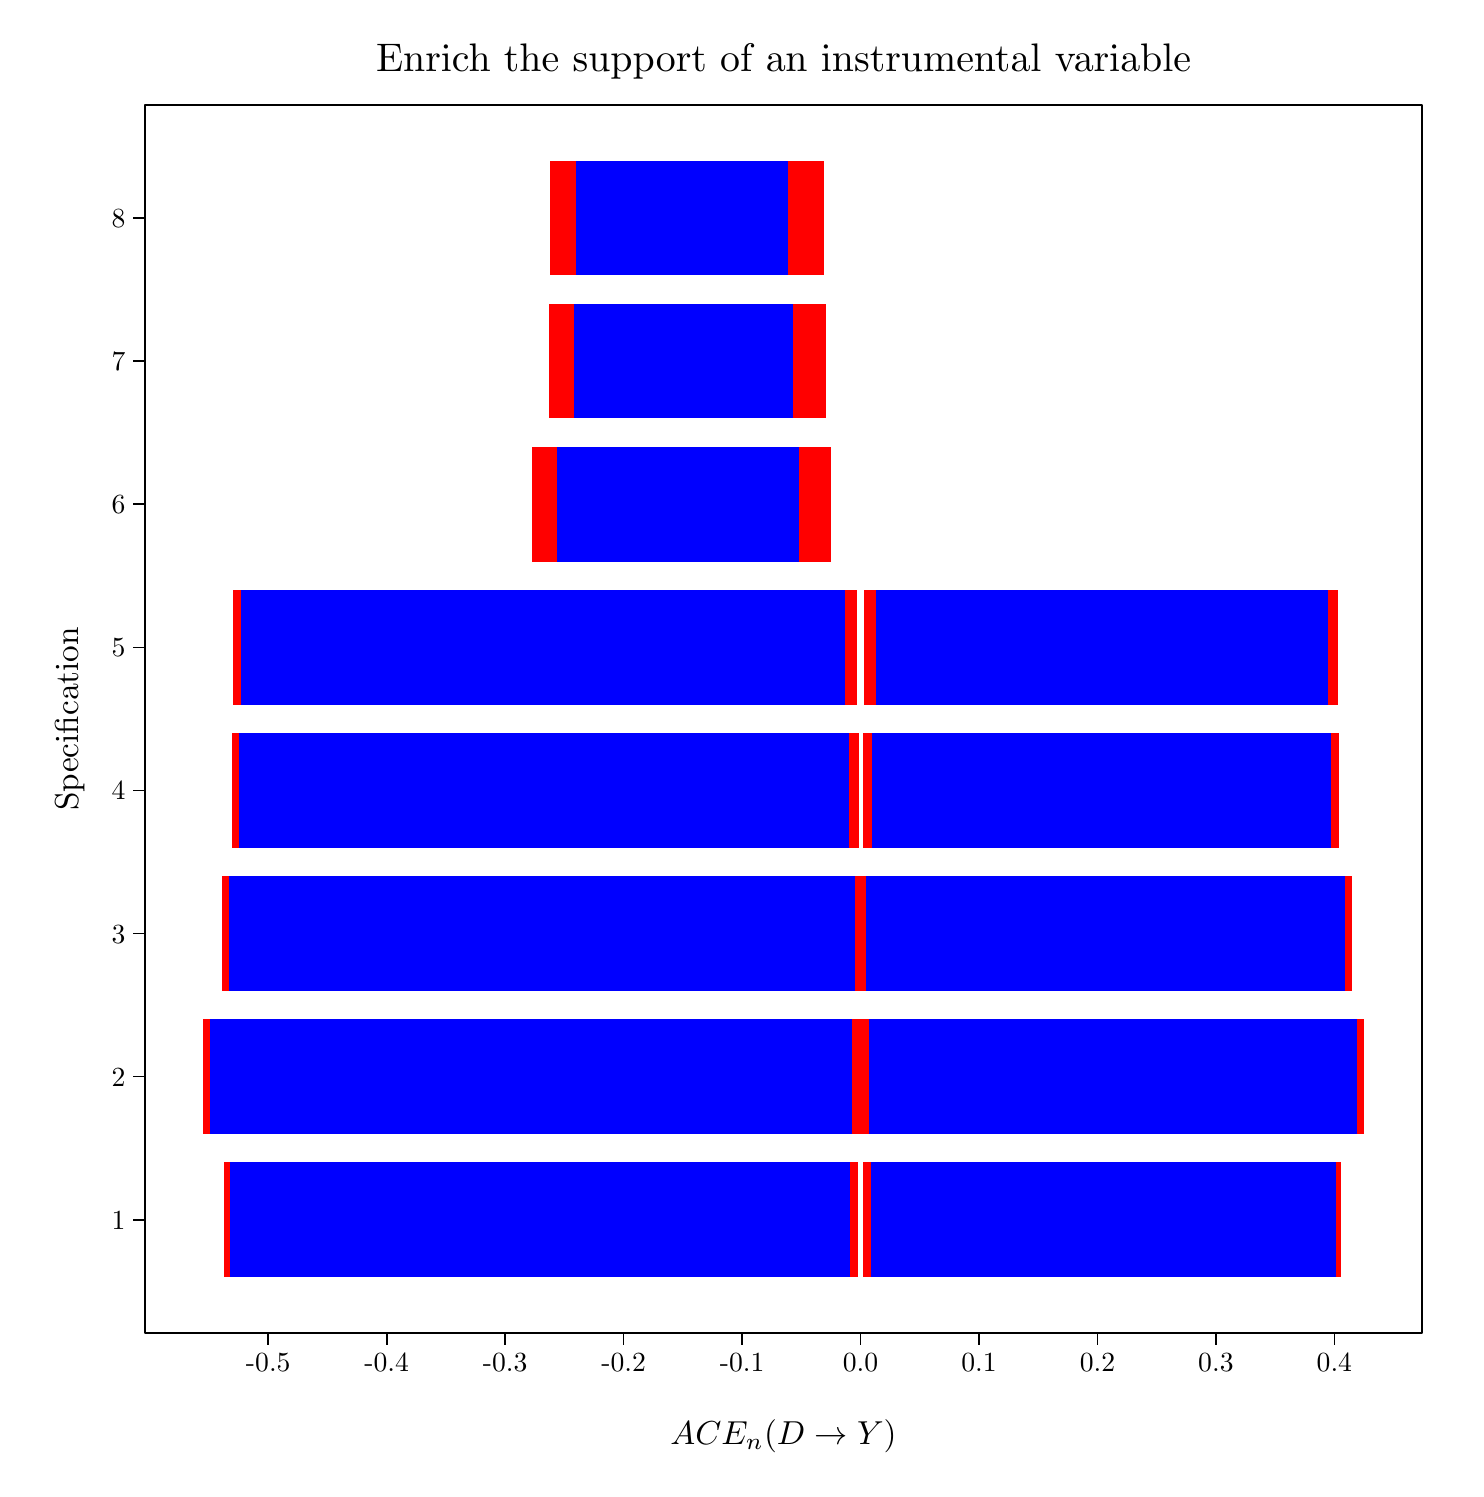
\begin{tikzpicture}[x=1pt,y=1pt]
\definecolor[named]{fillColor}{rgb}{1.00,1.00,1.00}
\path[use as bounding box,fill=fillColor,fill opacity=0.00] (-10,-15) rectangle (505.89,505.89);
\begin{scope}
\path[clip] (-10,-15) rectangle (505.89,505.89);
\definecolor[named]{fillColor}{rgb}{1.00,0.00,0.00}

\path[fill=fillColor] ( 61.10, 54.47) rectangle (290.10, 95.83);

\path[fill=fillColor] ( 53.40,106.17) rectangle (291.38,147.54);

\path[fill=fillColor] ( 60.24,157.88) rectangle (292.24,199.24);

\path[fill=fillColor] ( 63.67,209.58) rectangle (290.53,250.94);

\path[fill=fillColor] ( 64.10,261.28) rectangle (289.67,302.64);

\path[fill=fillColor] (172.39,312.98) rectangle (280.25,354.34);

\path[fill=fillColor] (178.38,364.68) rectangle (278.54,406.04);

\path[fill=fillColor] (178.81,416.38) rectangle (277.69,457.74);

\path[fill=fillColor] (291.81, 54.47) rectangle (464.74, 95.83);

\path[fill=fillColor] (290.53,106.17) rectangle (472.87,147.54);

\path[fill=fillColor] (289.67,157.88) rectangle (468.59,199.24);

\path[fill=fillColor] (291.81,209.58) rectangle (463.88,250.94);

\path[fill=fillColor] (292.24,261.28) rectangle (463.45,302.64);
\definecolor[named]{fillColor}{rgb}{0.00,0.00,1.00}

\path[fill=fillColor] ( 63.24, 54.47) rectangle (287.10, 95.83);

\path[fill=fillColor] ( 55.96,106.17) rectangle (287.96,147.54);

\path[fill=fillColor] ( 62.81,157.88) rectangle (288.82,199.24);

\path[fill=fillColor] ( 66.24,209.58) rectangle (286.68,250.94);

\path[fill=fillColor] ( 67.09,261.28) rectangle (285.39,302.64);

\path[fill=fillColor] (181.38,312.98) rectangle (268.70,354.34);

\path[fill=fillColor] (187.37,364.68) rectangle (266.56,406.04);

\path[fill=fillColor] (188.23,416.38) rectangle (264.85,457.74);

\path[fill=fillColor] (294.81, 54.47) rectangle (462.60, 95.83);

\path[fill=fillColor] (293.95,106.17) rectangle (470.30,147.54);

\path[fill=fillColor] (293.10,157.88) rectangle (466.02,199.24);

\path[fill=fillColor] (295.24,209.58) rectangle (460.89,250.94);

\path[fill=fillColor] (296.52,261.28) rectangle (460.03,302.64);
\definecolor[named]{drawColor}{rgb}{0.00,0.00,0.00}

\path[draw=drawColor,line width= 0.6pt,line join=round,line cap=round] ( 32.42, 34.31) rectangle (493.85,477.90);
\end{scope}
\begin{scope}
\path[clip] (-10,-15) rectangle (505.89,505.89);
\definecolor[named]{drawColor}{rgb}{0.00,0.00,0.00}

\path[draw=drawColor,line width= 0.6pt,line join=round] ( 32.42, 34.31) --
	( 32.42,477.90);
\end{scope}
\begin{scope}
\path[clip] (-10,-15) rectangle (505.89,505.89);
\definecolor[named]{drawColor}{rgb}{0.00,0.00,0.00}

\node[text=drawColor,anchor=base east,inner sep=0pt, outer sep=0pt, scale=  1.00] at ( 25.31, 71.71) {1};

\node[text=drawColor,anchor=base east,inner sep=0pt, outer sep=0pt, scale=  1.00] at ( 25.31,123.41) {2};

\node[text=drawColor,anchor=base east,inner sep=0pt, outer sep=0pt, scale=  1.00] at ( 25.31,175.11) {3};

\node[text=drawColor,anchor=base east,inner sep=0pt, outer sep=0pt, scale=  1.00] at ( 25.31,226.81) {4};

\node[text=drawColor,anchor=base east,inner sep=0pt, outer sep=0pt, scale=  1.00] at ( 25.31,278.51) {5};

\node[text=drawColor,anchor=base east,inner sep=0pt, outer sep=0pt, scale=  1.00] at ( 25.31,330.22) {6};

\node[text=drawColor,anchor=base east,inner sep=0pt, outer sep=0pt, scale=  1.00] at ( 25.31,381.92) {7};

\node[text=drawColor,anchor=base east,inner sep=0pt, outer sep=0pt, scale=  1.00] at ( 25.31,433.62) {8};
\end{scope}
\begin{scope}
\path[clip] (-10,-15) rectangle (505.89,505.89);
\definecolor[named]{drawColor}{rgb}{0.00,0.00,0.00}

\path[draw=drawColor,line width= 0.6pt,line join=round] ( 28.15, 75.15) --
	( 32.42, 75.15);

\path[draw=drawColor,line width= 0.6pt,line join=round] ( 28.15,126.85) --
	( 32.42,126.85);

\path[draw=drawColor,line width= 0.6pt,line join=round] ( 28.15,178.56) --
	( 32.42,178.56);

\path[draw=drawColor,line width= 0.6pt,line join=round] ( 28.15,230.26) --
	( 32.42,230.26);

\path[draw=drawColor,line width= 0.6pt,line join=round] ( 28.15,281.96) --
	( 32.42,281.96);

\path[draw=drawColor,line width= 0.6pt,line join=round] ( 28.15,333.66) --
	( 32.42,333.66);

\path[draw=drawColor,line width= 0.6pt,line join=round] ( 28.15,385.36) --
	( 32.42,385.36);

\path[draw=drawColor,line width= 0.6pt,line join=round] ( 28.15,437.06) --
	( 32.42,437.06);
\end{scope}
\begin{scope}
\path[clip] (-10,-15) rectangle (505.89,505.89);
\definecolor[named]{drawColor}{rgb}{0.00,0.00,0.00}

\path[draw=drawColor,line width= 0.6pt,line join=round] ( 32.42, 34.31) --
	(493.85, 34.31);
\end{scope}
\begin{scope}
\path[clip] (-10,-15) rectangle (505.89,505.89);
\definecolor[named]{drawColor}{rgb}{0.00,0.00,0.00}

\path[draw=drawColor,line width= 0.6pt,line join=round] ( 76.94, 30.04) --
	( 76.94, 34.31);

\path[draw=drawColor,line width= 0.6pt,line join=round] (119.74, 30.04) --
	(119.74, 34.31);

\path[draw=drawColor,line width= 0.6pt,line join=round] (162.54, 30.04) --
	(162.54, 34.31);

\path[draw=drawColor,line width= 0.6pt,line join=round] (205.35, 30.04) --
	(205.35, 34.31);

\path[draw=drawColor,line width= 0.6pt,line join=round] (248.15, 30.04) --
	(248.15, 34.31);

\path[draw=drawColor,line width= 0.6pt,line join=round] (290.96, 30.04) --
	(290.96, 34.31);

\path[draw=drawColor,line width= 0.6pt,line join=round] (333.76, 30.04) --
	(333.76, 34.31);

\path[draw=drawColor,line width= 0.6pt,line join=round] (376.56, 30.04) --
	(376.56, 34.31);

\path[draw=drawColor,line width= 0.6pt,line join=round] (419.37, 30.04) --
	(419.37, 34.31);

\path[draw=drawColor,line width= 0.6pt,line join=round] (462.17, 30.04) --
	(462.17, 34.31);
\end{scope}
\begin{scope}
\path[clip] (-10,-15) rectangle (505.89,505.89);
\definecolor[named]{drawColor}{rgb}{0.00,0.00,0.00}

\node[text=drawColor,anchor=base,inner sep=0pt, outer sep=0pt, scale=  1.00] at ( 76.94, 20.31) {-0.5};

\node[text=drawColor,anchor=base,inner sep=0pt, outer sep=0pt, scale=  1.00] at (119.74, 20.31) {-0.4};

\node[text=drawColor,anchor=base,inner sep=0pt, outer sep=0pt, scale=  1.00] at (162.54, 20.31) {-0.3};

\node[text=drawColor,anchor=base,inner sep=0pt, outer sep=0pt, scale=  1.00] at (205.35, 20.31) {-0.2};

\node[text=drawColor,anchor=base,inner sep=0pt, outer sep=0pt, scale=  1.00] at (248.15, 20.31) {-0.1};

\node[text=drawColor,anchor=base,inner sep=0pt, outer sep=0pt, scale=  1.00] at (290.96, 20.31) {0.0};

\node[text=drawColor,anchor=base,inner sep=0pt, outer sep=0pt, scale=  1.00] at (333.76, 20.31) {0.1};

\node[text=drawColor,anchor=base,inner sep=0pt, outer sep=0pt, scale=  1.00] at (376.56, 20.31) {0.2};

\node[text=drawColor,anchor=base,inner sep=0pt, outer sep=0pt, scale=  1.00] at (419.37, 20.31) {0.3};

\node[text=drawColor,anchor=base,inner sep=0pt, outer sep=0pt, scale=  1.00] at (462.17, 20.31) {0.4};
\end{scope}
\begin{scope}
\path[clip] (-10,-15) rectangle (505.89,505.89);
\definecolor[named]{drawColor}{rgb}{0.00,0.00,0.00}

\node[text=drawColor,anchor=base,inner sep=0pt, outer sep=0pt, scale=  1.20] at (263.13, -6.02) {$ACE_n(D\rightarrow Y)$};
\end{scope}
\begin{scope}
\path[clip] (-10,-15) rectangle (505.89,505.89);
\definecolor[named]{drawColor}{rgb}{0.00,0.00,0.00}

\node[text=drawColor,rotate= 90.00,anchor=base,inner sep=0pt, outer sep=0pt, scale=  1.20] at (  8.26,256.11) {Specification};
\end{scope}
\begin{scope}
\path[clip] (-10,-15) rectangle (505.89,505.89);
\definecolor[named]{drawColor}{rgb}{0.00,0.00,0.00}

\node[text=drawColor,anchor=base,inner sep=0pt, outer sep=0pt, scale=  1.44] at (263.13,489.95) {Enrich the support of an instrumental variable};
\end{scope}
\end{tikzpicture}
